\documentclass{article}

% if you need to pass options to natbib, use, e.g.:
%     \PassOptionsToPackage{numbers, compress}{natbib}
% before loading neurips_2018

% ready for submission
% \usepackage{neurips_2018}

% to compile a preprint version, e.g., for submission to arXiv, add add the
% [preprint] option:
%     \usepackage[preprint]{neurips_2018}

% to compile a camera-ready version, add the [final] option, e.g.:
\usepackage[final]{main}

% to avoid loading the natbib package, add option nonatbib:
%     \usepackage[nonatbib]{neurips_2018}
\usepackage[utf8]{inputenc} % allow utf-8 input
\usepackage[T1]{fontenc}    % use 8-bit T1 fonts
\usepackage{hyperref}       % hyperlinks
\usepackage{url}            % simple URL typesetting
\usepackage{booktabs}       % professional-quality tables
\usepackage{amsmath}       % general math
\usepackage{amsfonts}       % blackboard math symbols
\usepackage{nicefrac}       % compact symbols for 1/2, etc.
\usepackage{microtype}      % microtypography
\usepackage{booktabs}
\usepackage{subfig}
\usepackage{graphicx}

\title{DL: Assignment 2}

% The \author macro works with any number of authors. There are two commands
% used to separate the names and addresses of multiple authors: \And and \AND.
%
% Using \And between authors leaves it to LaTeX to determine where to break the
% lines. Using \AND forces a line break at that point. So, if LaTeX puts 3 of 4
% authors names on the first line, and the last on the second line, try using
% \AND instead of \And before the third author name.

\author{%
  Jonathan Mitnik \\
  MSc Artificial Intelligence\\
  University of Amsterdam\\
  \texttt{jonathan@student.uva.nl} \\
}

\begin{document}
% \nipsfinalcopy is no longer used
\maketitle

\begin{abstract}
    In this report, the main focus is to go through the assignment
\end{abstract}

\section{Recurrent Neural Networks}
\subsection*{1.1}
\subsubsection*{1.1.a}
The gradient can be calculated as follows:


% dsigma_j^2 / d_Xri
{\Large $\frac{\delta L^{(t)}}{\delta \textbf{W}_{ph}}$ }:
\boxed{\begin{aligned}
    \frac{\delta L^{(t)}}{\delta \textbf{W}_{ph}}
    &= \frac{\delta L^{(t)}}{\delta \hat{\textbf{y}}^{(t)}}
        \frac{\delta \hat{\textbf{y}}^{(t)}}{\delta \textbf{p}^{(t)}}
        \frac{\delta \textbf{p}^{(t)}}{\delta \textbf{W}_{ph}} \\
    &= \frac{\delta L^{(t)}}{\delta \hat{\textbf{y}}^{(t)}}
        \frac{\delta \hat{\textbf{y}}^{(t)}}{\delta \textbf{p}^{(t)}}
        \frac{\delta}{\delta \textbf{W}_{ph}} \textbf{W}_{ph} * h^{(t)} + b_{p} 
    &= \frac{\delta L^{(t)}}{\delta \hat{\textbf{y}}^{(t)}}
        \frac{\delta \hat{\textbf{y}}^{(t)}}{\delta \textbf{p}^{(t)}} h^{(t)}  \\
\end{aligned}}
\vspace{1cm}

\subsubsection*{1.1.b}
For the next gradient, we need to keep in mind the temporal and recursive nature. As such, we can define it as:
{\Large $\frac{\delta L^{(t)}}{\delta \textbf{W}_{hh}}$ }:
\boxed{\begin{aligned}
    \frac{\delta L^{(t)}}{\delta \textbf{W}_{hh}}
    &= \frac{\delta L^{(t)}}{\delta \hat{\textbf{y}}^{(t)}}
        \frac{\delta \hat{\textbf{y}}^{(t)}}{\delta \textbf{p}^{(t)}}
        \frac{\delta \textbf{p}^{(t)}}{\delta \textbf{h}^{(t)}} \\
        &= 
        \sum_{i=0}^{T=t}
        \frac{\delta L^{(t)}}{\delta \hat{\textbf{y}}^{(t)}}
        \frac{\delta \hat{\textbf{y}}^{(t)}}{\delta \textbf{p}^{(t)}}
        \frac{\delta \textbf{p}^{(t)}}{\delta \textbf{h}^{(t)}}
        \frac{\delta \textbf{h}^{(t)}}{\delta \textbf{h}_{i}}
        \frac{\delta \textbf{h}^{(i)}}{\delta \textbf{W}_{hh}} \\
    &=  \sum_{i=0}^{T=t}
        \frac{\delta L^{(t)}}{\delta \hat{\textbf{y}}^{(t)}}
        \frac{\delta \hat{\textbf{y}}^{(t)}}{\delta \textbf{p}^{(t)}}
        \frac{\delta \textbf{p}^{(t)}}{\delta \textbf{h}^{(t)}}
        \prod_{j=i+1}^{T} \Big( 
            \frac{\delta \textbf{h}^{(j)}}{\delta \textbf{h}_{j-1}}
        \Big)
        \frac{\delta \textbf{h}^{(i)}}{\delta \textbf{W}_{hh}} \\
\end{aligned}}
\vspace{1cm}

\subsection*{1.1.c}
There is a very clear distinction between the former formula and the latter: the derivative of the latter
does not depend on the previous time-steps. Essentially, the matrix mapping the output only depends on the last
hidden state. When you compare this to the recursive nature of $\frac{\delta L^{(t)}}{\delta \textbf{W}_{hh}}$, 
one important practical difference becomes clear: how "far" the gradient has to traverse to update the weights. For
$W_{ph}$, the gradient depends only on the latest hidden state, which means that the gradient and updates
generally are stronger. With $W_{hh}$, however, the jacobian product intuitievly either "explodes" the
gradient, or it weakens it, "vanishing" the gradient in the process the more time-steps we go back, due to 
its recursive nature.

\subsection*{1.2}
\subsubsection*{1.2.a}
Gates, go as follow:

\begin{enumerate}
    \item Input modulation gate: this gate is responsible for actually calculating new values that 
    are going to be eventually added to the cell-state. These values are modulated further with tanh,
    as to ensure that gradients remain stable by not exceeding 1 / -1 (as tanh does).
    \item Input gate: this gate acts as "differentiable" mask for the input modulation gate.
    It decides how much of the input modulation gate will be added on top of the current cell state.
    The sigmoid allows this "mask-like" functionality to be applied, ranging between 0 and 1.
    \item Forget gate: this gate is responsible for deciding how much of the previous cell state
    still remains (based on the current input and hidden state). It does so, again, by using
    sigmoids' range of 0 and 1 to decide whether to maintain nothing (0) or all (1).
    \item Output gate: this gate uses another "sigmoid-mask" to decide how much of the cell-state
    is used as hidden-state, possibly more short-term oriented. Before that, the cell-state
    is put through tanh to ensure that the value after its previous update is more stable again, max 1.
\end{enumerate}

\subsubsection*{1.2.b}
The number of parameters are $4 * \Big((N_{hidden} * N_{hidden}) + (N_{hidden} * N_{input}) 
+ N_{hidden}\Big) + (N_{hidden} * N_{output}) $.

\subsubsection*{1.3}
During training, the model was trained a number of times. To be more specific, the model was trained on three seeds (42, 1337 and 1994), with varying
sequence lengths eventually becoming 41 and 81 ((10, 20) * 4 + 2 -1). Both the training loss and training accuracy can be seen in the figure below, where
the standard deviation for every 10th step defines the "error-boundary", across seeds. Two noticeable differences occur. Whereas
sequences of 41 lenght eventually reach a proper convergence (across all seeds), sequences twice as long
still have a very high variance in both loss and and accuracy. However, this might be a simple shift of increased
variance that sequences of length 41 had (from timestep 500(=50*10) to 2000(=200*10)); if the model were to continue
to train, the model might reach similar convergence.

\begin{figure}[h]%
    \centering
    \subfloat[\centering LSTM accuracy averaged]{{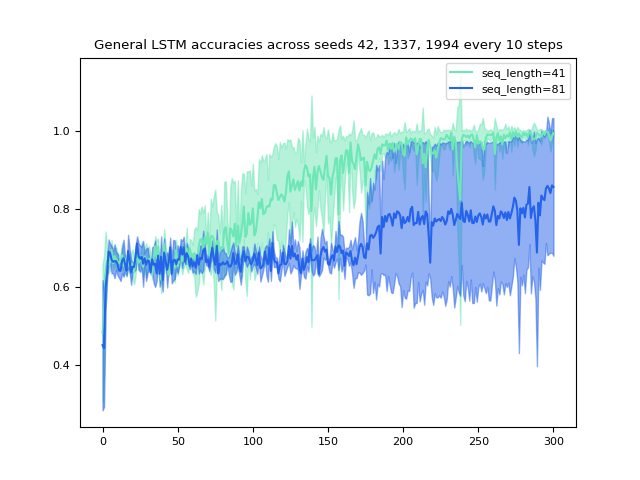
\includegraphics[width=6.5cm]{images/LSTM-plot-accs.png} }}%
    \qquad
    \subfloat[\centering LSTM loss averaged]{{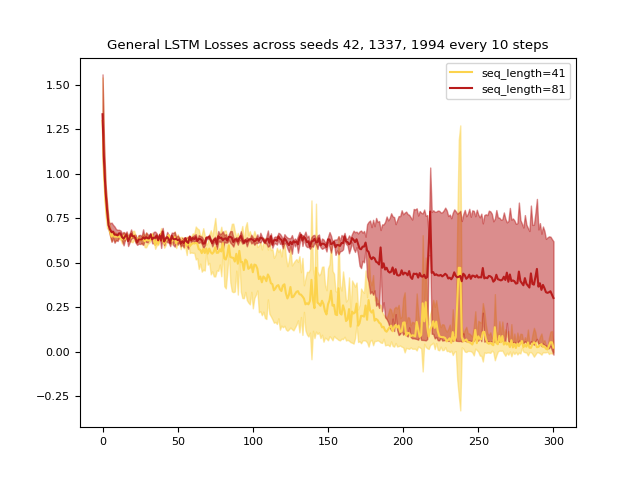
\includegraphics[width=6.5cm]{images/LSTM-plot-loss.png} }}%
    \caption{LSTM Performance over time: note, these are estimates stored every 10 steps of (3000), thus showing 300 recordings}%
    \label{fig:defaults}%
\end{figure}

\subsubsection*{1.4}
Now, with PeepLSTM, the results across sequence lengths look more similar to one another. The mean performance for 
both the longer sequence and shorter sequence seem to be much closer now, hinting at the idea that the peepholes
may make models more robust in general for longer sequences (even if the variance is still relatively high). What's
more, the signal averages seem more noisy, indicating slightly less stable predictions in general (notice both
losses and accuracies seem to be contain more discord). The true power of the peephole LSTM is mostly visible
when looking at the general increase in performance speed for lenght 81: where the vanilla seemed to plateau for
a while (likely due to the output gate being closed), Peephole LSTMS bypass some of the problems by provind this extra signal.

\begin{figure}[h]%
    \centering
    \subfloat[\centering PeepLSTM accuracy averaged]{{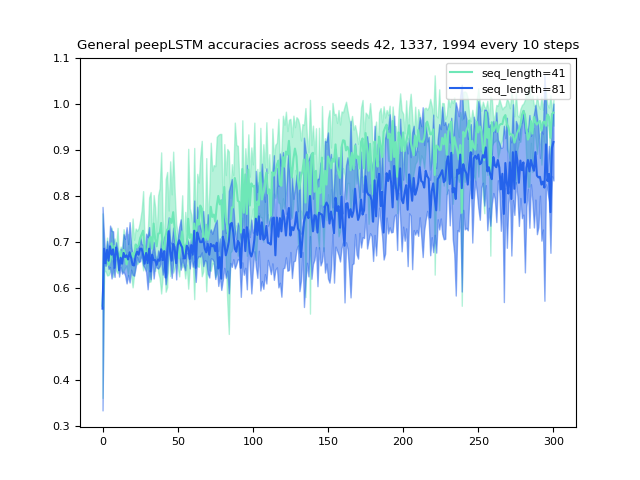
\includegraphics[width=6.5cm]{images/peepLSTM-plot-accs.png} }}%
    \qquad
    \subfloat[\centering PeepLSTM loss averaged]{{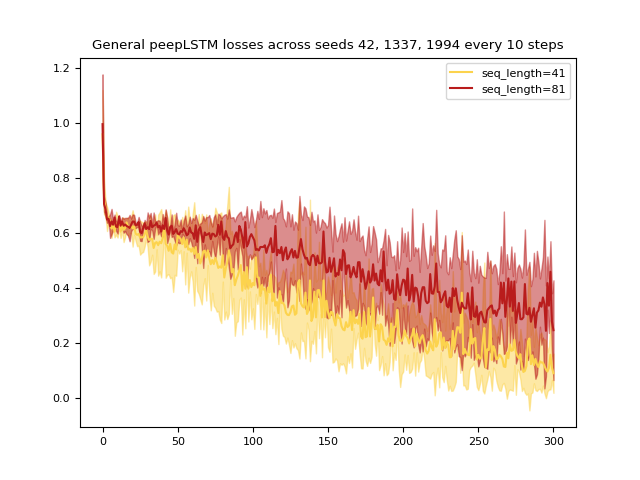
\includegraphics[width=6.5cm]{images/peepLSTM-plot-loss.png} }}%
    \caption{PeepLSTM Performance over time: note, these are estimates stored every 10 steps of (3000), thus showing 300 recordings}%
    \label{fig:defaults}%
\end{figure}


\section{Recurrent Nets as Generative Model}
test

\section{Graph Neural Networks}
\subsection{GCN Forward Layer}
\subsubsection*{3.1.a}
The structure of the graph can be found represented in $\hat{A}$, 
which is composed of the Diagonals $\tilde{D}$ (meaning how many neighbours a node has) 
and $\tilde{A}$, representing the edges of the nodes (the adjacency matrix). 
This multiplication will instruct which neighbouring nodes will receive 
the message formed by the $W^{(l)}$-projection of $H^{(l)}$ from the prior layer, 
and how much of it (this is the normalization step). This message as such is shared among neighbours,
and propagated through the layers.

\subsubsection*{3.1.b}
One major problem, is when nodes have the same neighbours: because the input for all nodes
are shared equally across neighbours, including a node's own input, the output will lose
the distinguishability of a node's meaning. An alternative to this, would be to use \emph{attention}
to let a model learn the weighed averages of neighbours rather than treating them equally.

\subsubsection*{3.2.a}
$$ \tilde{A} = 
    \left( \begin{matrix} 0 & 1 & 0 & 0 & 1 & 1 \\ 1 & 0 & 0 & 1 & 0 & 0 \\ 0 & 0 & 0 & 1 & 0 & 0 \\ 0 & 1 & 1 & 0 & 0 & 1 \\ 1 & 0 & 0 & 0 & 0 & 0 \\ 1 & 0 & 0 & 1 & 0 & 0 \end{matrix} \right)
    + \left( \begin{matrix} 1 & 0 & 0 & 0 & 0 & 0 \\ 0 & 1 & 0 & 0 & 0 & 0 \\ 0 & 0 & 1 & 0 & 0 & 0 \\ 0 & 0 & 0 & 1 & 0 & 0 \\ 0 & 0 & 0 & 0 & 1 & 0 \\ 0 & 0 & 0 & 0 & 0 & 1 \end{matrix} \right)
    =
    \left( \begin{matrix} 1 & 1 & 0 & 0 & 1 & 1 \\ 1 & 1 & 0 & 1 & 0 & 0 \\ 0 & 0 & 1 & 1 & 0 & 0 \\ 0 & 1 & 1 & 1 & 0 & 1 \\ 1 & 0 & 0 & 0 & 1 & 0 \\ 1 & 0 & 0 & 1 & 0 & 1 \end{matrix} \right) $$

\subsubsection*{3.2.b}
The number of updates this would take is 4. The first update would go from C to D, then this
would be passed both to F and B, then on the third update they both pass some part of C to A, which
on the fourth update will be passed to E.

\subsection{Graph Attention Networks}
What we need to add to the existing formula, is obviously some coefficient to express the attention
relationship between i and j. This is introduces an MLP \emph{a} which maps the concatenation of i and
j to a relationship, a LeakyRelu which ensures that attention remains dependent on the query, and a
softmax to scale the attention to become a probability distribution. 

$$
    h_i^{(l+1)} = \sigma \Big(
        \sum_{j \in N(i)} \frac{exp(LeakyRelu(a * [Wh_i || Wh_j]))}{\sum_{k \in N_i} exp(LeakyRelu(a * [Wh_i || Wh_k]))} * W^{(l)} h_j^{(l)}
    \Big )
$$

\subsection{Applications of GNNs}
A first example could be for instance improving a recommender system with knowledge graph information,
as detailed in \cite{guo2020survey}. For instance, when recommending movies to a user, a movies can utilize
as connections such as other movies a leading actor played in, or perhaps movies a friend enjoyed as well. 
This is in general an edge-level task.
A node-level use-case could be enhancing embeddings via concatenation, such as is done 
in \cite{DBLP:journals/corr/abs-1909-08402}. When classifying books (nodes), one could classify these
with BERT embeddings, but also use related structural information such as author.

\subsection{Comparing and Combining GNNs and RNNs}

\subsubsection*{3.4.a}
Any spatial information that is not 1-dimensional likely benefits more form GNNs than RNNs. In 
its traditional form, RNNs do not consider more than a linear dimension. Therefore, images will work 
better with a GNN that accounts for its entire neighbourhood. However, GNNs are less robust when
it comes to particular order, such as an important sequence of text: RNNs traverse these sequences
with an emphasis on order, therefor being able to parse translation between languages better.

\subsubsection*{3.4.b}
In \cite{fernandes2020structured}, a summarization task is discussed, where a bit of text is processed
using traditional RNN encoder style. This is then enriched by inserting these token representation into
a gated GNN, which borrows gating techniques as proposed by the LSTMs. The GNNs can then utilize 
supervised relationships of these tokens/embeddings, and pool the resulting node-transformations
into a decodable summary.


\bibliography{main}{}
\bibliographystyle{plain}

\end{document}